\chapter{Resultados}

%\lipsum[1-1]

%POR QUE O PROBLEMA DA MCHILA NÃO ENTROU?
%FAÇA COMPARAÇÃO COM FORÇA-BRUTA! UM DAS SOLUÇÕES APRESENTADAS DEMORA QUASE 5 HORAS!!!
O primeiro conjunto de experimentos foi realizado para minimizar o Custo Total de Rotas (CTR), ou seja, a soma da rota de cada equipe. Ao comparar as soluções, a solução, que possui o menor custo total, é considerada a melhor. Este cenário pode ser aplicado à vida real quando pretendemos reduzir a quantidade total de rotas de entrega em vez de priorizar o equilíbrio de trabalho.

O segundo conjunto de experimentos visou minimizar a Rota Mais Longa (RML) das soluções mantendo os mesmos valores dos parâmetros no primeiro cenário. Esse caso é adequado para situações reais quando priorizamos o equilíbrio entre as rotas individuais (\textit{workbalance}) em vez da soma total das rotas.

% ---
\section{Resultados sem Otimizadores Globais}
\label{sec-resultados-taco}
% ---

Foi utilizado a abordagem TACO com regras do ACS para otimização da instância vista na Seção 5 para quatro entregadores. Foram realizados dois experimentos: minimização do custo total das soluções e minimização da maior rota individual das soluções.

A Tabela \ref{tab:resultado-taco} mostra o tempo médio de execução do algoritmo (em horas) para a instância. Este valor foi obtido a partir da média do tempo gasto para executar os 1000 ciclos TACO nas 30 execuções do algoritmo, por um dia útil.

\begin{table}[htb]
    \centering
    \caption{Resultados para o TACO sem Otimizadores Globais} \label{tab:resultado-taco}
\begin{tabular}{|c|c|c|c|c|c|c|c|}
\hline
\multicolumn{8}{|c|}{Média de 30 simulações com 1000 iterações}                                                            \\ \hline
\multicolumn{4}{|c|}{Minimizando o Custo Total das Rotas (CTR)} & \multicolumn{4}{c|}{Minimizando a Rota Mais Longa (RML)} \\ \hline
CTR           & D.P.          & RML            & D.P.           & CTR           & P.D.         & RML         & D.P.        \\ \hline
1.8           & 0.25          & 0.721          & 0.003          & 1.223         & 0.050        & 0.756       & 0.012       \\ \hline
\end{tabular}
\end{table}

O TACO apresentou resultados satisfatórios para as duas variações do MTSP: minimizar o custo total da solução e minimizar o custo da maior rota de solução individual (Tabela \ref{tab:resultado-taco}). Os pequenos valores dos desvios padrão nas duas tabelas confirmam a robustez do algoritmo ao gerar soluções com custos próximos da média das 30 execuções. Embora a RL esteja sendo minimizada, o TCR varia ao longo das iterações, conforme observado no Figura \ref{fig:resultados-convergencia-taco-tcr}. A mesma situação ocorre quando a TACO minimiza o TCR (ver Figura \ref{fig:resultados-convergencia-taco-rml}). Tendo isso em mente, ainda há espaço para melhorias nos resultados de ambos os objetivos.

\begin{figure}[htb]
    \centering
    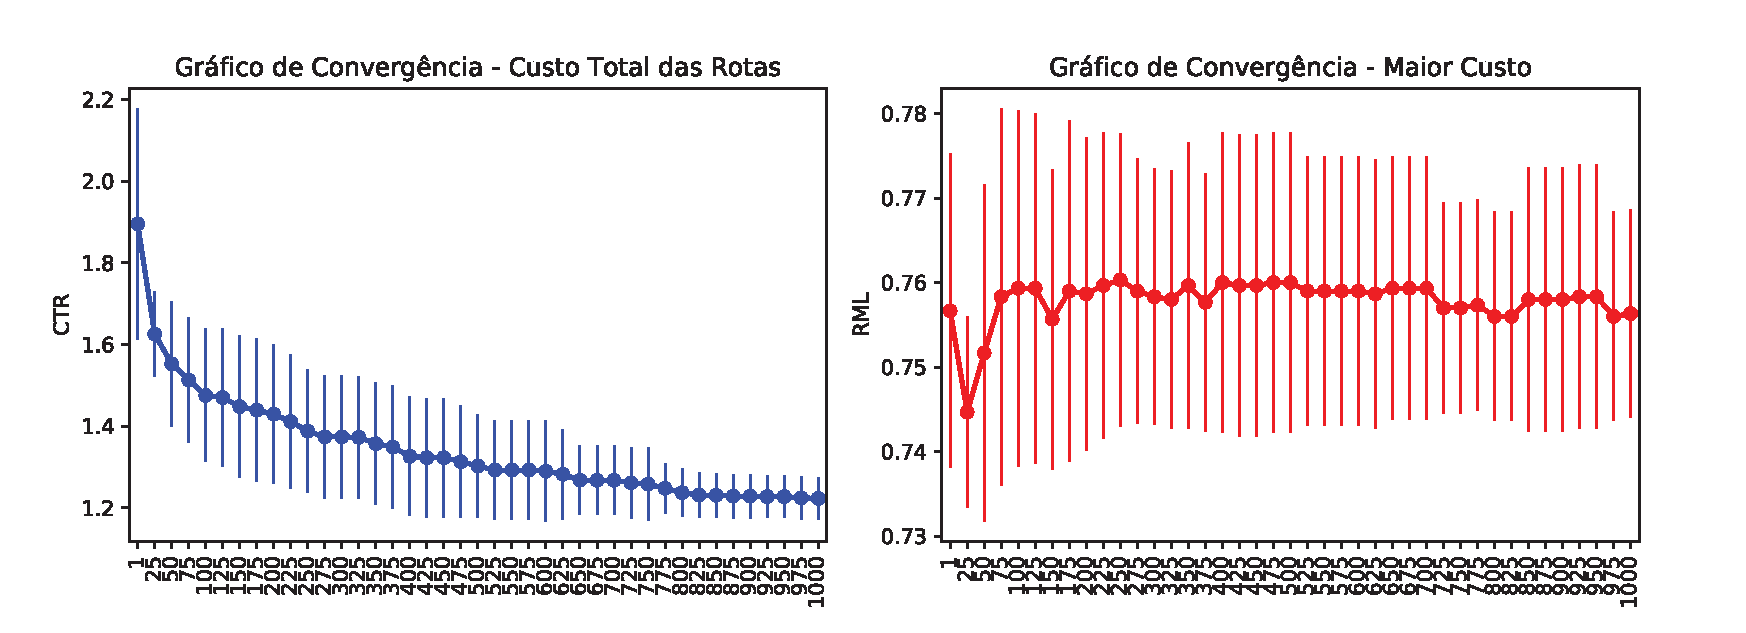
\includegraphics[width=\textwidth]{imagens/convergence-totalcost-taco.eps}
    \caption{Curva de convergência quando minimizado o CTR} \label{fig:resultados-convergencia-taco-tcr}
\end{figure}

\begin{figure}[htb]
    \centering
    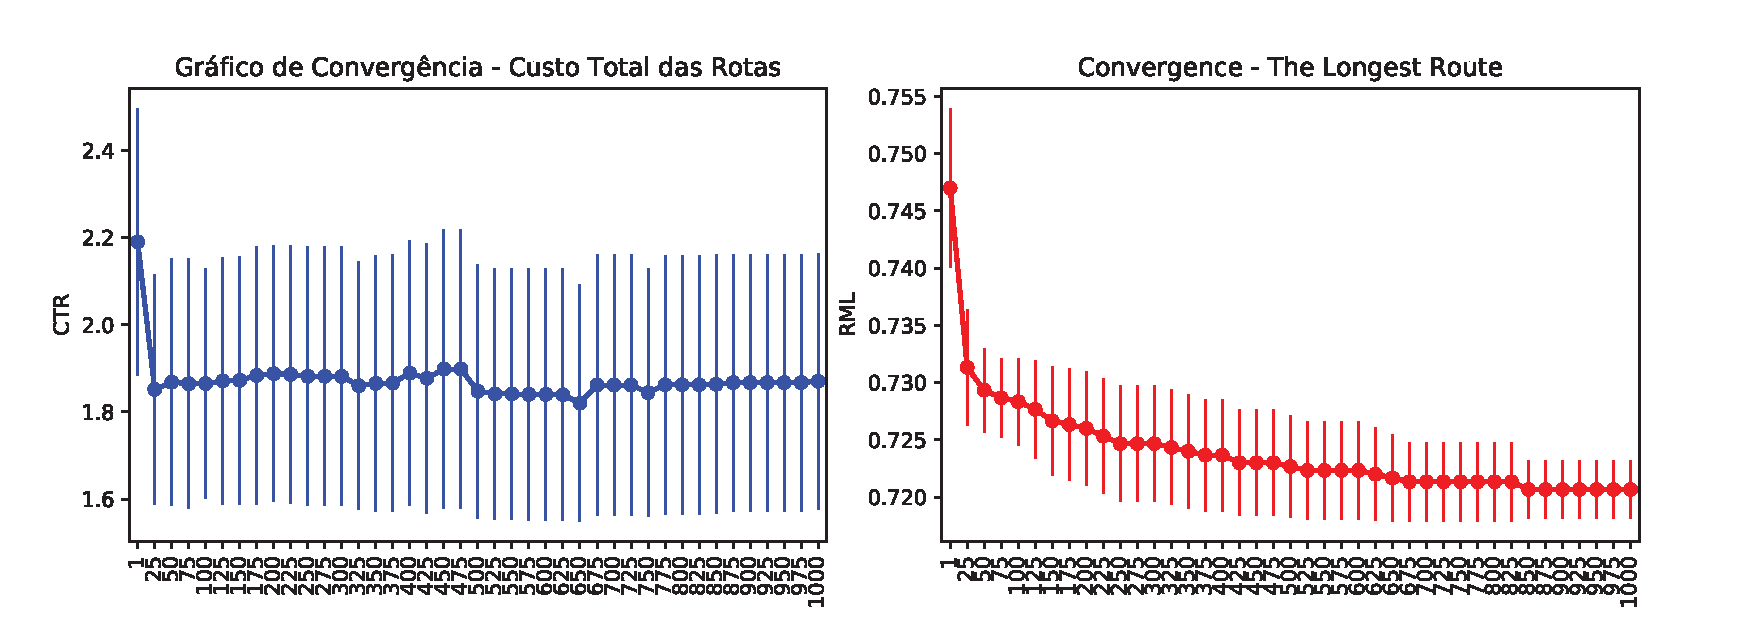
\includegraphics[width=\textwidth]{imagens/convergence-maxcost-taco.eps}
    \caption{Curva de convergência quando minimizado RML} \label{fig:resultados-convergencia-taco-rml}
\end{figure}

% ---
\section{Resultados com Otimizadores Globais}
\label{sec-resultados-fss-pso}
% ---

Os experimentos realizados com o otimizador externo mostraram melhores resultados para ambos os cenários, mostrados nas Tabelas \ref{tab:resultado-fsstaco} e \ref{tab:resultado-psotaco}. Comparando as Tabelas \ref{tab:resultado-taco} e \ref{tab:resultado-fsstaco}, o FSS tem uma melhora melhor ao minimizar a rota mais longa em comparação ao algoritmo base. Esse resultado é devido à capacidade do FSS de explorar o espaço de pesquisa. Além disso, o FSS apresenta um desvio padrão menor, o que corrobora a sua robustez.

\begin{table}[htb]
    \centering
    \caption{Resultados para TACO com FSS sendo o Otimizador Global} \label{tab:resultado-fsstaco}
\begin{tabular}{|c|c|c|c|c|c|c|c|}
\hline
\multicolumn{8}{|c|}{Média de 30 simulações com 1000 iterações}                                                            \\ \hline
\multicolumn{4}{|c|}{Minimizando o Custo Total das Rotas (CTR)} & \multicolumn{4}{c|}{Minimizando a Rota Mais Longa (RML)} \\ \hline
CTR             & D.P.           & RML           & D.P.         & CTR          & D.P.         & RML          & D.P.        \\ \hline
1.0797          & 0.002          & 0.747         & 0            & 1.944        & 0.335        & 0.719        & 0.001       \\ \hline
\end{tabular}
\end{table}

\begin{figure}[htb]
    \centering
    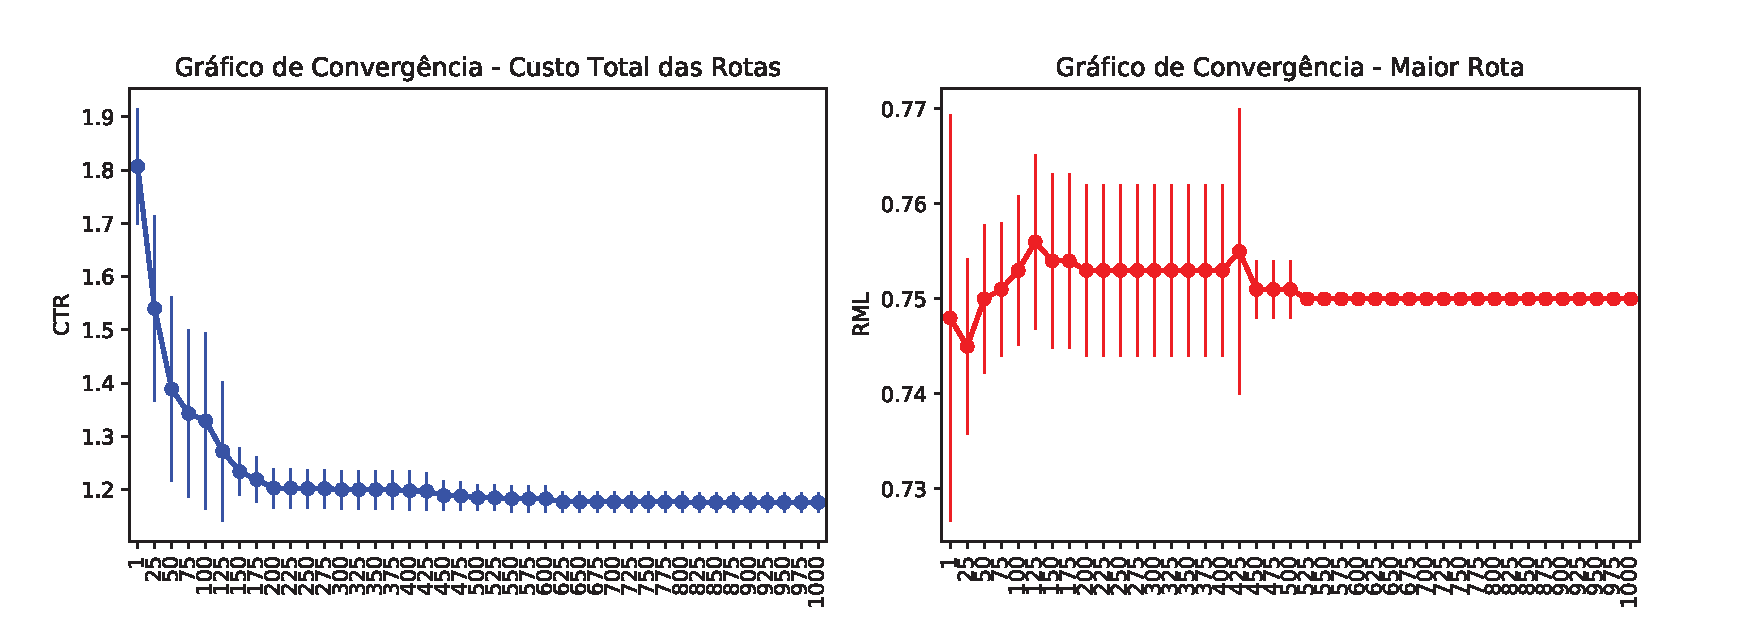
\includegraphics[width=\textwidth]{imagens/convergence-totalcost-fsstaco.eps}
    \caption{Curva de convergência FSS-TACO quando minimizado o CTR} \label{fig:resultados-convergencia-fss-tcr}
\end{figure}

\begin{figure}[htb]
    \centering
    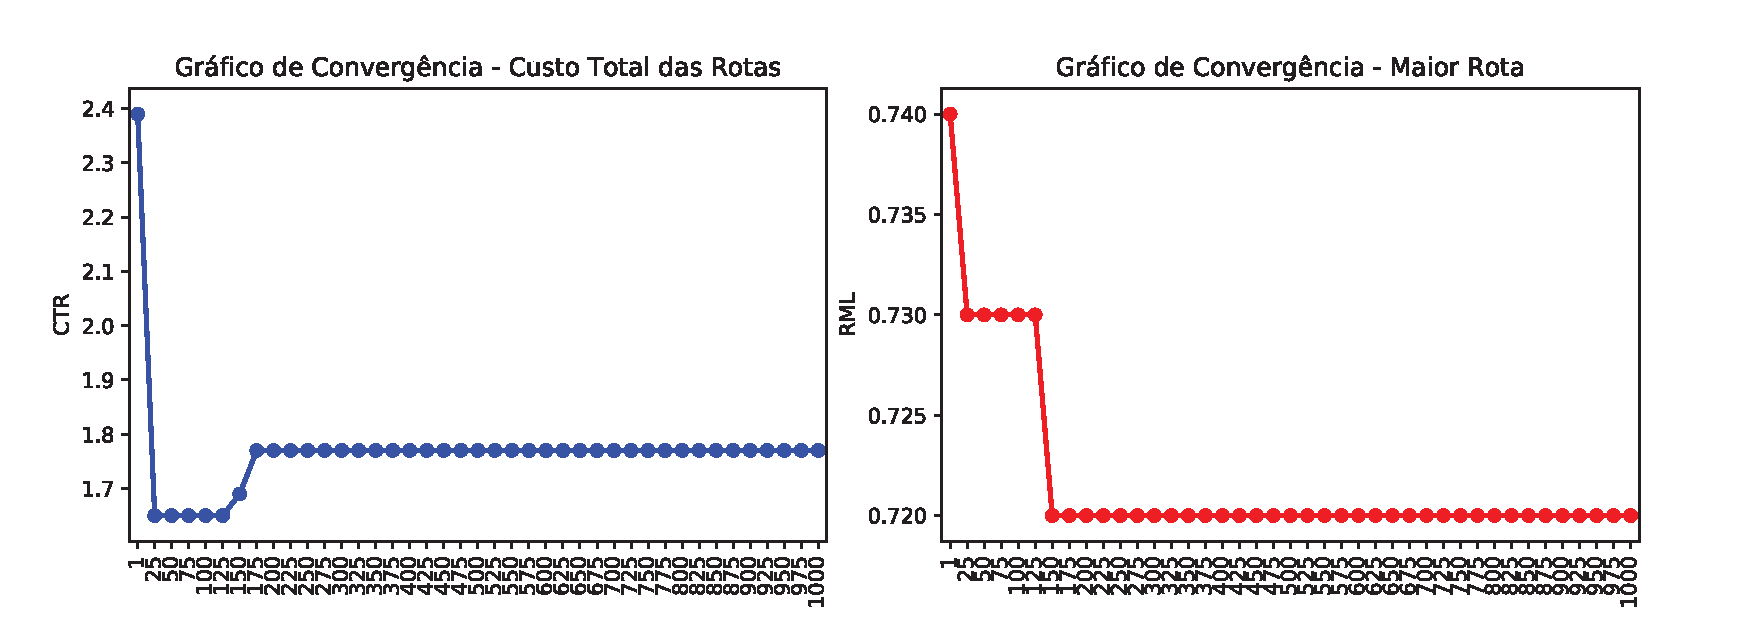
\includegraphics[width=\textwidth]{imagens/convergence-maxcost-fsstaco.eps}
    \caption{Curva de convergência FSS-TACO quando minimizado a RML} \label{fig:resultados-convergencia-fss-rml}
\end{figure}

PSO também teve melhores resultados em comparação com abordagem TACO sem otimizadores externos (ver Tabela \ref{tab:resultado-psotaco}). Seu desvio padrão também mostra a robustez e eficácia ao otimizar TCR e LR.

\begin{table}[htb]
    \centering
    \caption{Resultados para TACO com PSO sendo o Otimizador Global} \label{tab:resultado-psotaco}
\begin{tabular}{|c|c|c|c|c|c|c|c|}
\hline
\multicolumn{8}{|c|}{Média de 30 simulações com 1000 iterações}                                                            \\ \hline
\multicolumn{4}{|c|}{Minimizando o Custo Total das Rotas (CTR)} & \multicolumn{4}{c|}{Minimizando a Rota Mais Longa (RML)} \\ \hline
CTR            & D.P.           & RML           & D.P.          & CTR          & D.P.         & RML          & D.P.        \\ \hline
1.115          & 0.032          & 0.750         & 0.003         & 2.048        & 0.333        & 0.720        & 0.005       \\ \hline
\end{tabular}
\end{table}

\begin{figure}[htb]
    \centering
    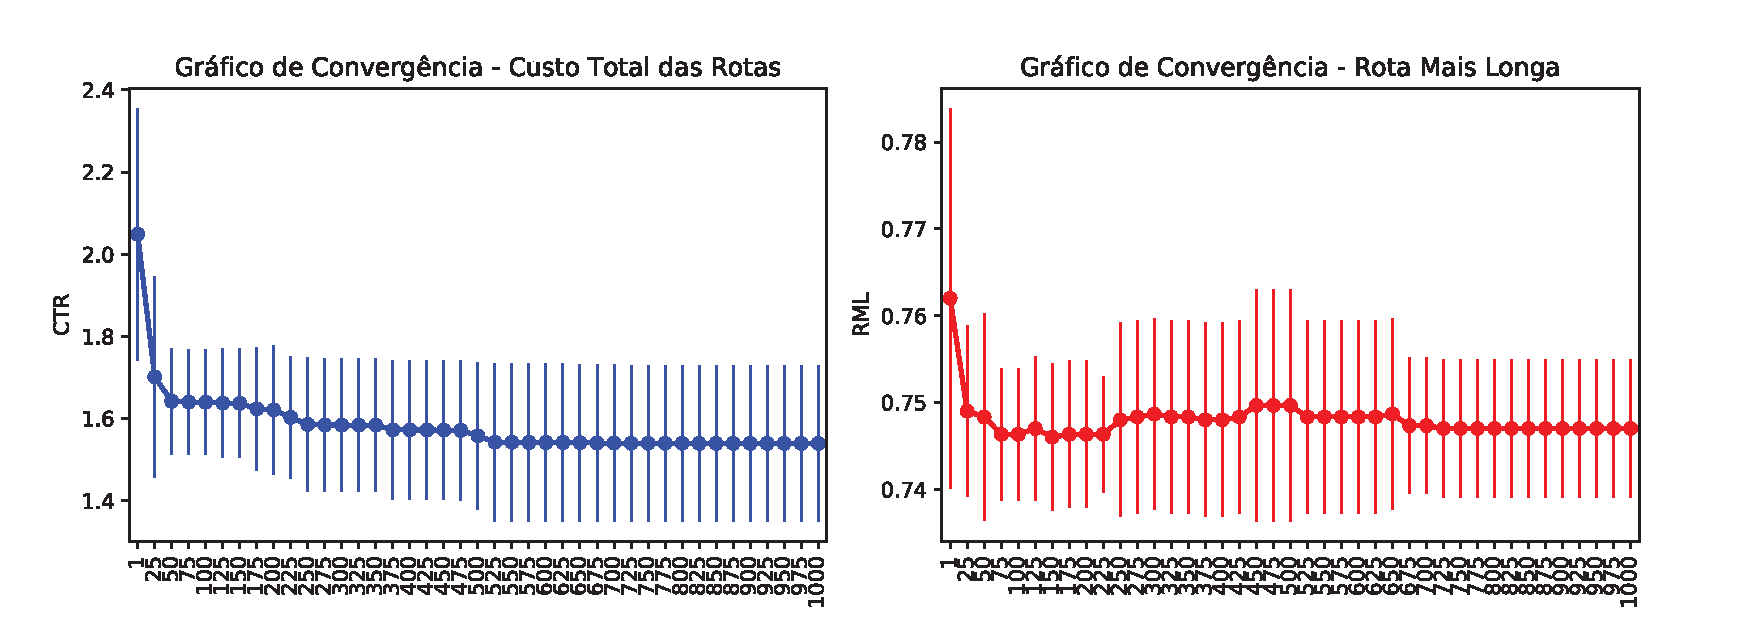
\includegraphics[width=\textwidth]{imagens/convergence-totalcost-psotaco.eps}
    \caption{Curva de convergência PSO-TACO quando minimizado o CTR} \label{fig:resultados-convergencia-pso-tcr}
\end{figure}

\begin{figure}[htb]
    \centering
    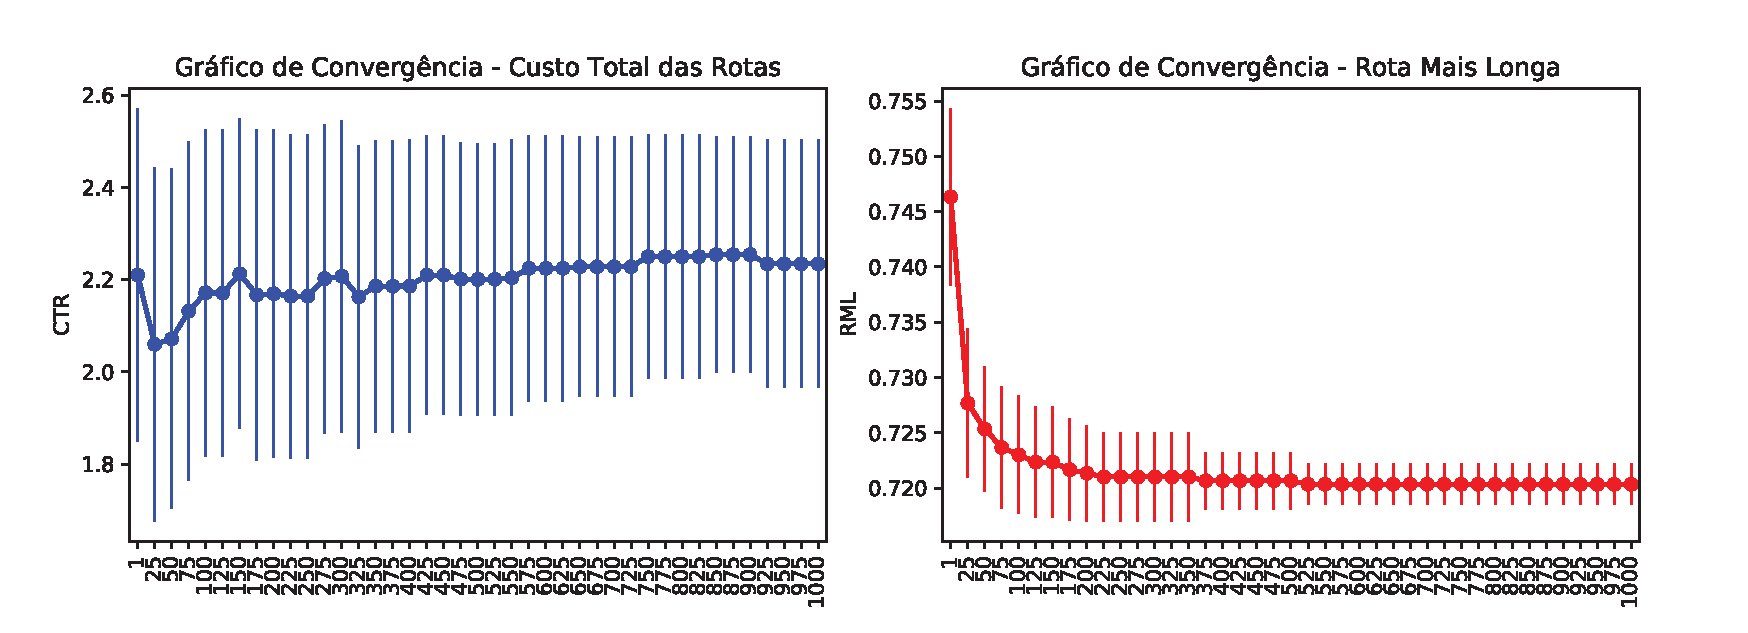
\includegraphics[width=\textwidth]{imagens/convergence-maxcost-psotaco.eps}
    \caption{Curva de convergência PSO-TACO quando minimizado a RML} \label{fig:resultados-convergencia-pso-rml}
\end{figure}

Os experimentos realizados com o otimizador externo mostraram melhores resultados para ambos os cenários, mostrados nas Tabelas \ref{tab:resultado-fsstaco} e \ref{tab:resultado-psotaco}. Conforme apresentado nas Tabelas \ref{tab:resultado-taco} e \ref{tab:resultado-fsstaco}, o FSS tem uma melhora melhor de minimizar a rota mais longa em comparação ao algoritmo base. Esse resultado é devido à capacidade do FSS de explorar o espaço de pesquisa. Além disso, o FSS apresenta um desvio padrão menor, o que corrobora sua robustez.

% ---
\section{Comparativo entre os experimentos}
\label{sec-resultados-taco}
% ---

Todos os resultados anteriores são compilados na Tabela \ref{tab:resultado-comparison} para um melhor entendimento deles. Comparando as três abordagens, o FSS obteve melhores resultados ao minimizar tanto o CTR quanto a RML. Também teve o menor resultado com um desvio padrão próximo de zero. Como visto na Figura \ref{fig:resultados-convergencia}, em ambos os cenários, o FSS convergiu mais cedo do que o PSO e o algoritmo de base. Os resultados do PSO foram melhores que os resultados do algoritmo de base e convergiram mais cedo do que o TACO como esperado.

\begin{figure}[htb]
    \centering
    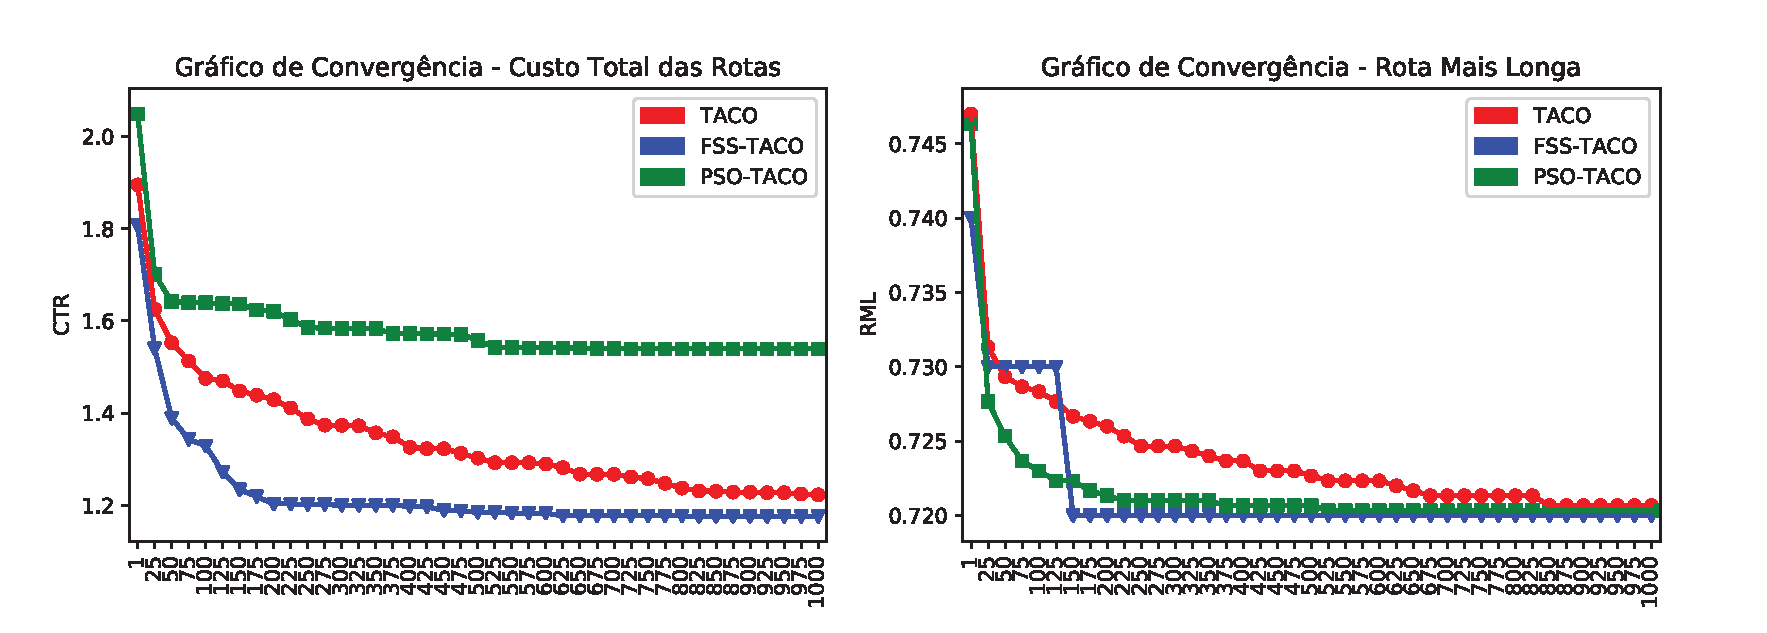
\includegraphics[width=\textwidth]{imagens/convergence-approaches.eps}
    \caption{Comparação entre as convergências de TACO, FSS-TACO e PSO-TACO} \label{fig:resultados-convergencia}
\end{figure}

% Please add the following required packages to your document preamble:
% \usepackage{multirow}
\begin{table}[htb]
    \centering
    \caption{Comparação entre resultados com 30 simulações independentes} \label{tab:resultado-comparison}
\begin{tabular}{|c|c|c|c|c|c|c|c|c|}
\hline
\multirow{2}{*}{Abordagem} & \multicolumn{4}{l|}{Minimizando o CTR}           & \multicolumn{4}{l|}{Minimizando a RML}          \\ \cline{2-9} 
                            & CTR             & D.P.           & RML   & D.P.  & CTR   & D.P.  & RML            & D.P.           \\ \hline
TACO                       & 1.8             & 0.25           & 0.721 & 0.003 & 1.223 & 0.050 & 0.756          & 0.012          \\ \hline
FSS-TACO                   & \textbf{1.0797} & \textbf{0.002} & 0.747 & 0     & 1.944 & 0.335 & \textbf{0.719} & \textbf{0.001} \\ \hline
PSO-TACO                   & 1.115           & 0.032          & 0.750 & 0.003 & 2.048 & 0.333 & 0.720          & 0.005          \\ \hline
\end{tabular}
\end{table}

A Figura \ref{fig:resultados-boxplot} mostra o desvio padrão para ambos os CTR e RML. Ao minimizar o CTR, podemos notar que os resultados do TACO variam mais do que o FSS e PSO. Por outro lado, PSO tem a menor variação de seus resultados. Ao minimizar a RML, vale ressaltar que para todas as abordagens (TACO, FSS e PSO) existe uma pequena ou nenhuma variação entre seus resultados.

\begin{figure}[htb]
    \centering
    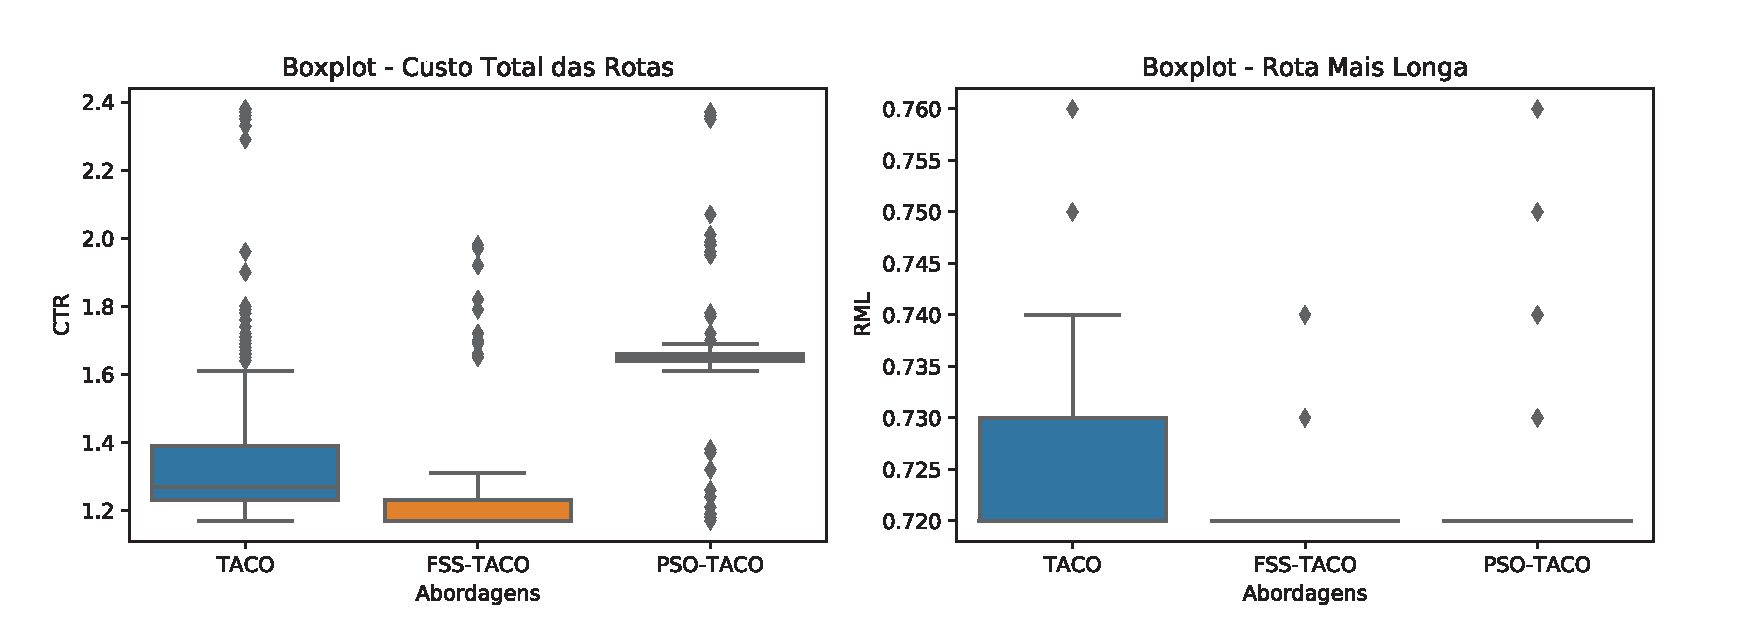
\includegraphics[width=\textwidth]{imagens/boxplot-approaches.eps}
    \caption{Boxplot com os desvios padrões da minimização do CTR e da RML} \label{fig:resultados-boxplot}
\end{figure}

% ---
\section{Tempos de Execução dos Algoritmos}
\label{sec-resultados-tempo}
% ---

A Tabela \ref{tab:resultado-tempo} apresenta o tempo médio de execução do algoritmo para cada instância. Este valor foi obtido a partir da média do tempo gasto para execução dos 1000 ciclos de cada abordagem nas 30 execuções independente do algoritmo.

% Please add the following required packages to your document preamble:
% \usepackage{multirow}
\begin{table}[htb]
    \centering
    \caption{Tempo médio de execução de 1.000 ciclos de TACO, FSS-TACO e PSO-TACO} \label{tab:resultado-tempo}
    \begin{tabular}{|c|c|c|}
    \hline
    \multirow{2}{*}{Abordagem} & Minimizando o CTR & Minimizando a RML \\ \cline{2-3} 
                               & Tempo Médio (ms)  & Tempo Médio (ms)  \\ \hline
    TACO                       & 618,53            & 609,73            \\ \hline
    FSS-TACO                   & 16945914,10       & 15701984,33       \\ \hline
    PSO-TACO                   & 5218562,20        & 5161234,17        \\ \hline
    \end{tabular}
\end{table}

Quanto aos tempos de execução do algoritmo, mostrados na Tabela \ref{tab:resultado-tempo}, verifica-se que para a instância experimentada, foram gastos em media aproximadamente 0,6 segundo para execução dos 1000 ciclos do algoritmo, que representam um tempo aceitável para o problema em estudo. Entretanto, ao comparar a abordagem utilizando os OGs PSO e FSS o tempo médio de execução passa 1 hora e 4 horas, respectivamente. Em ambos os cenários de otimização (minimizando CTR ou RML), a abordagem com OG sendo PSO é mais rápida do que o OG sendo o FSS. Ao levar em consideração o tempo que os pedidos são feitos ao CAF (pedidos aceitos até às 8h da manhã), o PSO leva vantagem pois o tempo de processamento é menor, levando a um menor tempo na distribuição dos medicamentos.

% ---
\section{Análise dos Resultados Parciais para o MOFSS-TACO}
\label{sec-resultados-tempo}
% ---

%COLOCAR OS RESULTADOS FINAIS DO MOFSS-TACO
Os resultados parciais para o MOFSS sendo o OG do algoritmo base (ver Tabela \ref{tab:resultado-mofss}) se mostram bastante interessantes. Ao minimizar simultaneamente CTR e RML, o MOFSS consegue resultados menores que o TACO sem otimizador externo, tendo em vista os valores otimizados do TACO de forma mono-objetiva como visto na Tabela \ref{tab:resultado-taco}. Entretanto, para os resultados parciais não são menores quando comparados as abordagens PSO-TACO e FSS-TACO. Todavia, deve ser levado em consideração que os objetivos CTR e RML estão sendo minimizados de forma simultânea o que garante um tempo de execução menor dos que os outros dois.

\begin{table}[htb]
    \centering
    \caption{Resultados para TACO com MOFSS sendo o Otimizador Global} \label{tab:resultado-mofss}
    \begin{tabular}{|c|c|c|c|}
    \hline
    \multicolumn{4}{|c|}{Média de 10 simulações com 1000 iterações} \\ \hline
    \multicolumn{4}{|c|}{Minimizando CTR e RML}                     \\ \hline
    CTR            & D.P.          & RML            & D.P.          \\ \hline
    1,435          & 0,29          & 0,731          & 0,011         \\ \hline
    \end{tabular}
    \end{table}

Ao fim de cada execução, a abordagem MOFSS-TACO gera um conjunto de soluções ótimas não-dominadas. Como o problema não tem grande complexidade, ao final de cada execução independente gera um conjunto com quatro soluções não dominadas.

\section{Discussão dos Resultados}

O resultado do desvio padrão (D.P.) se mostra satisfatório confirmando a robustez do algoritmo para os experimentos contemplando somete o TACO. Comparado com a minimização dos dois objetivos, a minimização da RML foi inferior na minimização do CTR. Essa otimização proporciona um número maior de entregas pelos entregadores visto que o custo da rota individual é balanceado de modo a não sobrecarregar ou ocasionar ociosidade em um dos entregadores. Com os entregadores realizando mais entregas em menos tempo, essa técnica é mais favorável quando o custo total do deslocamento não é o objetivo, mas sim a quantidade de entregas por cada entregador.

Vale ressaltar que, na minimização do CTR, a carga não é distribuída de maneira uniforme para os entregadores podendo um ou mais entregadores ficar com sobrecarga ou ocioso dependendo da configuração. Já na minimização da RML, focado em minimizar a maior rota individual, distribuindo a carga de maneira uniforme para todos os entregadores.

Ao comparar os resultados, sem e com OGs e otimização mono-objetivo, é possível perceber o bom desempenho da abordagem FSS-TACO em face das abordagens TACO e PSO-TACO. Entretanto, o seu uso se torna inviável, dependendo da situação, por requerer um tempo de execução superior aos das outras abordagens presentes na comparação. Para uma abordagem multi-objetiva, o MOFSS sendo o OG do algoritmo base, mostra resultados parciais interessantes visto que obteve resultados melhores para CTR e RML se comparado aos resultados do algoritmo base. Como a instância construída para este trabalho não possui grande complexidade, a Curva de Pareto, com as soluções ótimas, se restringe a quatro soluções não-dominadas.